%%---------------------------------------------------------------------
%	Preamble
%	AMS gruppe 12
%	AMS F18
%---------------------------------------------------------------------
\documentclass[12pt,fleqn,a4paper]{article}
\usepackage[utf8]{inputenc}
\usepackage[danish]{babel}
\usepackage[top=2.5cm, left=2cm, right=2cm, bottom=2.5cm]{geometry}
\usepackage{graphicx}
\usepackage[bottom]{footmisc}
\usepackage{framed}
\usepackage{caption}
\usepackage{float}
\usepackage{mdframed}
\usepackage{listings}
\usepackage{color}
\usepackage[T1]{fontenc}
\usepackage{amsmath,amsfonts,amsthm} % Math packages
\usepackage{array}
\usepackage{wrapfig}
\usepackage{multirow}
\usepackage{tabu}
\usepackage{longtable}
\usepackage{lastpage}
\usepackage{fancyhdr}
\usepackage[compact]{titlesec}
\usepackage[table,xcdraw]{xcolor}
\usepackage{arydshln}
\usepackage[isbn,issn,url]{dk-bib}
\usepackage[toc,page]{appendix}
\usepackage{url}
\def\UrlBreaks{\do\/\do-}

\definecolor{mygreen}{RGB}{28,172,0} % color values Red, Green, Blue
\definecolor{mylilas}{RGB}{170,55,241}
\renewcommand{\lstlistingname}{Kodeudsnit}
\tabulinesep=3mm

\setcounter{secnumdepth}{2}
\setcounter{tocdepth}{2}

\setlength{\parindent}{0mm} %intet indryk
\setlength{\parskip}{3mm} 	%linjeskift v. afsnit

% Ændring af enumerize og itemize 
\usepackage{enumitem} % @http://ctan.org/pkg/enumitem
\setlist[itemize]{topsep=0pt, itemsep=0.5pt}
\setlist[enumerate]{topsep=0pt, itemsep=0.5pt}

%afstand omkring sections
\titlespacing{\section}{0pt}{5mm}{0pt}
\titlespacing{\subsection}{0pt}{2mm}{0pt}
\titlespacing{\subsubsection}{0pt}{2mm}{0pt}

\usepackage{arydshln}
%aryd
\setlength\dashlinedash{3pt}
\setlength\dashlinegap{4pt}

\lstset{language=C++,
	breaklines=true,
	keywordstyle=\color{blue},
	stringstyle=\color{red},
	commentstyle=\color{mygreen},
	morecomment=[l][\color{magenta}]{\#}
}

%header & footer
\makeatletter
\pagestyle{fancy}
\fancypagestyle{plain}{}
\renewcommand{\chaptermark}[1]{\markboth{#1}{}}
\setlength{\headheight}{35pt}
\fancyfoot{} % clear all fields
\fancyfoot[R]{Side \thepage\ af \pageref{LastPage}}
\fancyhead{} % clear all fields
\fancyhead[L]{
\includegraphics[clip, trim = 0 0 240pt 0, height=30pt]{Figur/IHA_AU_logo.png}}
\fancyhead[R]{Forår 2018}
\fancyhead[C]{Anvendte Microcontroller Systemer}
\renewcommand{\headrulewidth}{0pt}

\def\thickhrulefill{\leavevmode \leaders \hrule height 1.2ex \hfill \kern \z@}
\def\@makechapterhead#1{
  \vspace*{10\p@}%
  {\parindent \z@ \centering \reset@font
        \thickhrulefill\quad 
        \scshape\bfseries\textit{\@chapapp{}  \thechapter}  
        \quad \thickhrulefill
        \par\nobreak
        \vspace*{10\p@}%
        \interlinepenalty\@M
        \hrule
        \vspace*{10\p@}%
        \Huge \bfseries #1 \par\nobreak
        \par
        \vspace*{10\p@}%
        \hrule
        \vskip 40\p@
  }}

\usepackage{tcolorbox}
\definecolor{mycolor}{rgb}{0.122, 0.435, 0.698}% Rule colour
\makeatletter
\newcommand{\mybox}[1]{%
	\setbox0=\hbox{#1}%
	\setlength{\@tempdima}{\dimexpr\wd0+13pt}%
	\begin{tcolorbox}[colframe=mycolor,boxrule=0.5pt,arc=4pt,
		left=6pt,right=6pt,top=6pt,bottom=6pt,boxsep=0pt]
		#1
	\end{tcolorbox}
}
\makeatother

\graphicspath{ {Figur/} }


%Se Kodeudsnit \ref{lstlisting:generel_kode}

%\captionof{lstlisting}{Generelle egenskaber for koden til fremstilling af diverse figure i matlab} 
%\label{lstlisting:generel_kode}
%\vspace{5mm} %5mm vertical space
%
%\subsection{Kode til lyd i forhold til tiden}
%\begin{framed}
%\begin{center}
%\begin{lstlisting}
%figure('name','trafikstoejen i fuld laengde'); clf
%subplot(211);
%plot(t,s_sound_left)
%xlabel('Tid (sek)')
%ylabel('Signalstyrke')
%title('Trafikstoej set i forhold til tiden')
%grid on
%hold on
%\end{lstlisting}
%\end{center}
%\end{framed}




%\begin{document}

\section{GUI}
Dette afsnit beskriver, hvordan GUI'et er designet, implementeret og testet.
GUI'et består af klasserne MainWindow, ActiveChoice og my\_qlabel, samt filen guimessages.h.

\subsection{MainWindow}
GUI'et består blandt andet af skærmklassen, MainWindow. 
MainWindow kan befinde sig i to tilstande: "Menu" og "Drive". 
På figurerne nedenfor (figur \ref{fig:Menuscreen} og \ref{fig:Drivescreen}) ses hhv. menuskærmen og køreskærmen.

\begin{figure} [H]
	\centering
	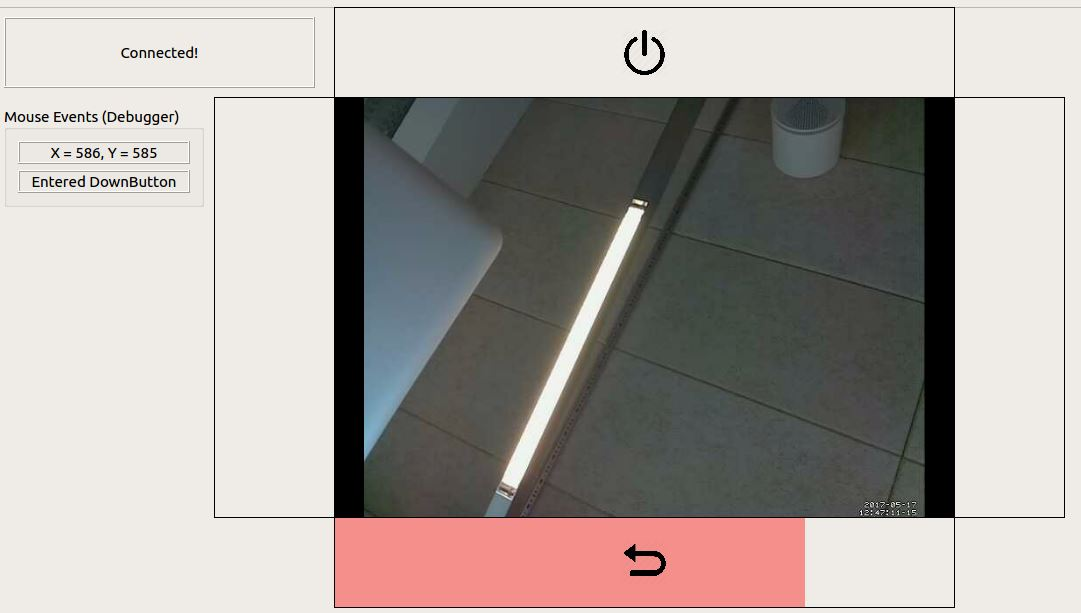
\includegraphics[width = \textwidth]{figur/Menuscreen.JPG}
	\caption{Skærmbillede af menuskærmen}
	\label{fig:Menuscreen}
\end{figure}

\begin{figure} [H]
	\centering
	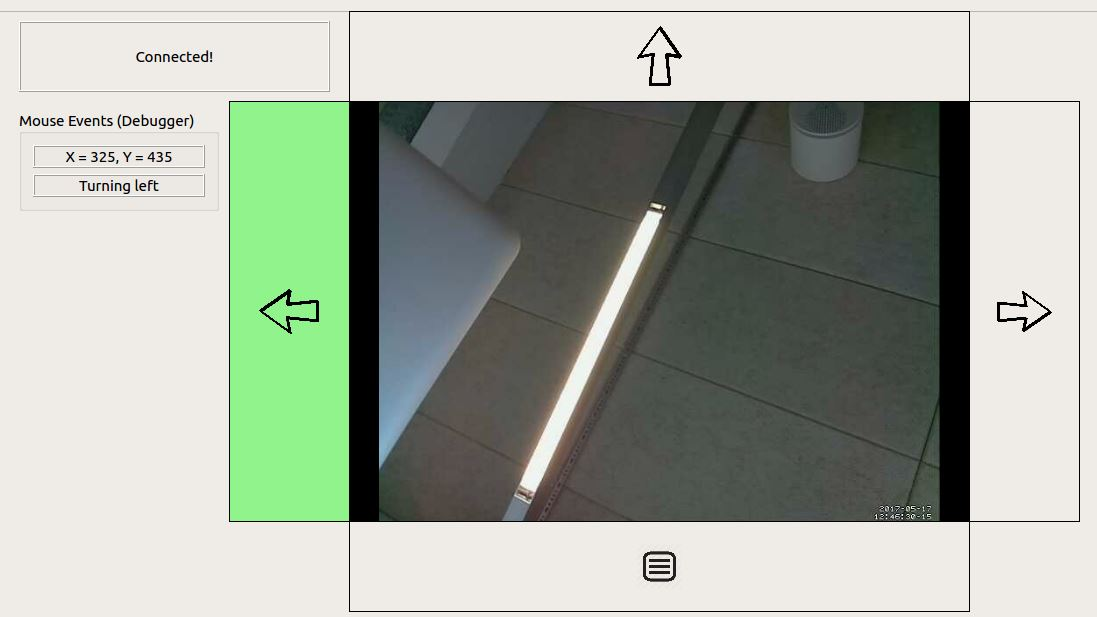
\includegraphics[width = \textwidth]{figur/Drivescreen.JPG}
	\caption{Skærmbillede af køreskærmen}
	\label{fig:Drivescreen}
\end{figure}

For at opsætte robotkameraets videostream på GUI'et kaldes funktionen 
\begin{lstlisting}
void MainWindow::SetupVideoStream()
\end{lstlisting}

Denne metode forbinder robottens videostream til GUI'et. 
Metoden opsætter videostreamet ved brug af klassen QMediaPlayer. 
Klassen får fat i streamet ved brug af Kontrolenhedens IP adresse samt portnummeret således:
\begin{lstlisting}
player->setMedia(QUrl("http://10.3.141.1:8081"),NULL);
\end{lstlisting}

Metoden kaldes fra MainWindows constructor.

For at opsætte valgfelterne rundt omkring videostreamet kaldes funktionen 
\begin{lstlisting}
void MainWindow::SetupButtonConnections()
\end{lstlisting}

Denne metode forbinder de events fra klassen my\_qlabel (beskrevet i næste afsnit) til MainWindow-klassens funktioner: 
\begin{lstlisting}
void MainWindow::Mouse_current_pos();
void MainWindow::Mouse_Pressed()
void MainWindow::Mouse_Left()
void MainWindow::Mouse_Entered()
\end{lstlisting}
\newpage
\subsection{my\_qlabel}
De fire valgfelter på GUI'et består af denne klasse. Klassen gør det muligt at registrere events på valgfelterne. 
Herunder ses de fire events, som emitterer et signal til MainWindows Mouse-funktioner.

\begin{lstlisting}
void my_qlabel::mouseMoveEvent(QMouseEvent*){emit Mouse_Pos();}
void my_qlabel::mousePressEvent(QMouseEvent*){emit Mouse_Pressed();}
void my_qlabel::leaveEvent(QEvent*){emit Mouse_Left();}
void my_qlabel::enterEvent(QEvent*){emit Mouse_Entered();}
\end{lstlisting}

\subsection{ActiveChoice}
Denne klasse håndterer 'Aktivt valg' funktionaliteten. Klassen består af to metoder: 
\begin{lstlisting}
void ActiveChoice::StartTimer(QWidget *)
void ActiveChoice::StopTimer()
\end{lstlisting}

StartTimer metoden kaldes, når der registreres et enterEvent på et valgfelt. 
Dette kunne for eksempel være, når brugeren bevæger cursoren hen over menufeltet.
Når der registreres et enterEvent, kaldes metoden og valgfeltet sendes med som parameter. 
Metoden starter en timer, der kalder UpdateProgressBarSlot() med et 20ms interval, hvorved procesbaren begynder at blive fyldt op. 
Derudover startes en anden timer, der efter 2 sekunder genererer et klik-event på det respektive valgfelt.

StopTimer funktionen stopper begge timere og nulstiller procesbaren. 
Metoden kaldes når der registreres et leaveEvent, hvilket sker når cursoren fjernes fra valgfeltet.

\subsection{GUIMessages}
Denne klasse indeholder de forskellige beskeder GUI'et kan sende videre til PC'ens main.
Klassen indeholder to structs, der bruges som beskeder: \textit{PowerOffInd} og \textit{RobotControlInd}. 
PowerOffInd indikerer, at valgfeltet Dvale er valgt. 
RobotControlInd indeholder information om, hvilket kontrol-valgfelt der er valgt. Når et respektivt valgfelt er valgt tilføjes en af disse message-structs til en besked-kø oprettet af PC'ens main program.

På figur \ref{GUI_STM} ses et tilstandsdiagram over GUI'et.

\begin{figure} [H]
	\centering
	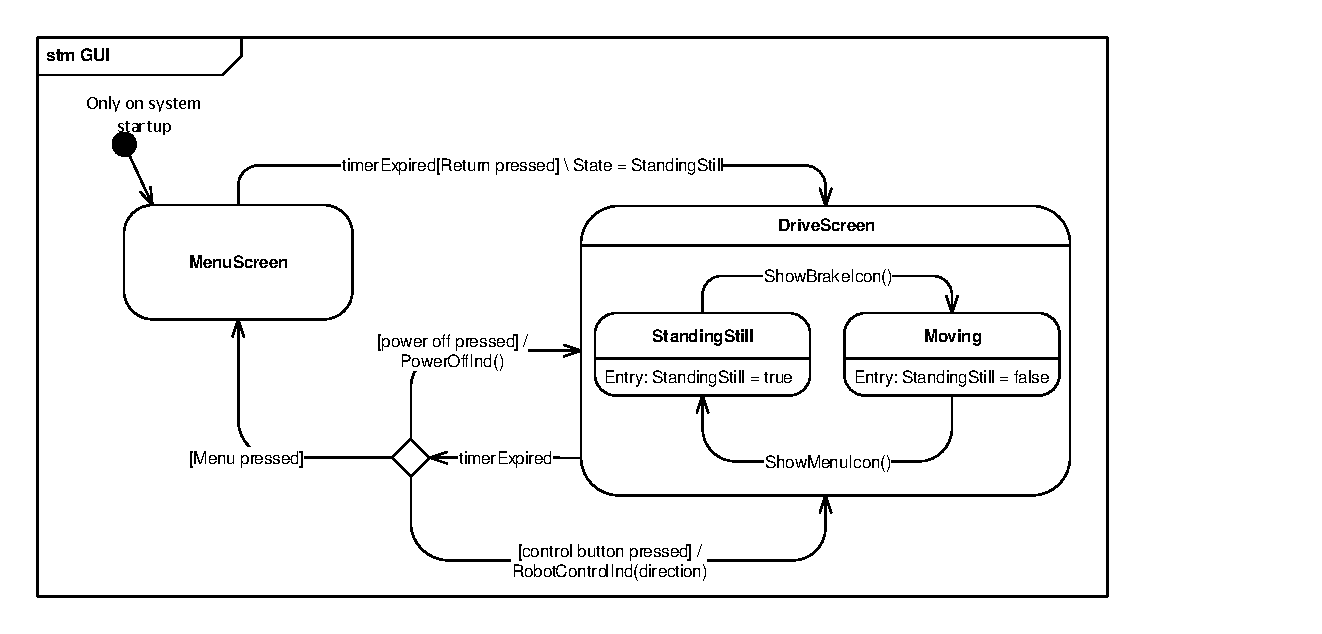
\includegraphics[clip, trim = 0cm 0cm 3cm 0.5cm, width = \textwidth]{figur/STM_GUI.pdf}
	\caption{GUI tilstandsdiagram}
	\label{GUI_STM}
\end{figure}


\subsection{Enhedstest}
Ved test af GUI'et testes om, det er muligt at flytte cursoren ved brug af MainWindow funktionen MoveCursorToCoordinates(x, y). 
Herefter testes om GUI'ets fire valgfelter kan registrere et aktivt valg og signalere dette til Main tråden.\\
Det testes også at videostreamet kan vises på GUI'et. Testen kan ses på bilag \ref{appendix:BilagGUIEnhedstest}.

Efter udførsel af testen kan det konkluderes, at GUI'et opfylder kravene. 
	
%\end{document}